\chapter{The JUNO experiment}

The first idea of a medium baseline (~60 km) experiment, was explored in 2008 where it was demonstrated that the Neutrino Mass Ordering (NMO) could be determined by a medium baseline experiment if $\sin^2(2\theta_{13}) > 0.005$ without requirements on accurate information of reactor antineutrino spectra and the value of $\Delta m_{32}^2$. \cite{zhan_determination_2008}
It was shown that for value of \todo{Stopped here for now. See V.L. JUNO chapter before getting back here}


The JUNO (Jiangmen Underground Neutrino Observatory) is a neutrino detection experiment located in China. Its main objective is the determination of the mass ordering at the 3-4$\sigma$ level in 6 years of data taking \cite{an_neutrino_2016}.

\section{Neutrinos physics in JUNO}

As said before, the main goals of JUNO are the determination of the NMO and the precise measurements of the oscillation parameters $\Delta m_{21}^2$, $\sin^2 2\theta_{12}$, $\Delta m_{32}^2$ and, with less precision, $\sin^2\theta_{13}$. \todo{Might remove this line if enough precision in precedent chapter/section}

\subsection{Reactor neutrino oscillation for NMO and precise measurements}

Previous works \cite{zhan_determination_2008,  zhan_experimental_2009} shows that oscillation parameters and the NMO can be observed by looking at the $\bnue$ disappearance spectrum coming from medium baseline nuclear reactor. This disappearance probability can be expressed as \cite{an_neutrino_2016} :
\begin{equation*}
  P(\bnue \rightarrow \bnue) = 1 - \sin^2 2\theta_{12} c^4_{13} sin^2 \frac{\Delta m^2_{21}L}{4E} - \sin^2 2\theta_{13} \bigg[ c_{12}^2 \sin^2 \frac{\Delta m_{31}^2 L}{4E} + s^2_{12} \sin^2 \frac{\Delta m_{32}^2 L}{4E} \bigg]
\end{equation*}
Where $s_{ij} = \sin \theta_{ij}$, $c_{ij} = \cos \theta_{ij}$, $E$ is the $\bnue$ energy and $L$ is the baseline.
We can see the sensitivity to the NMO in the dependency to $\Delta m_{32}^2$ and $\Delta m^2_{31}$ causing a phase shift of the spectrum (Figure \ref{fig:juno-spectrum-oscillation}).
By carefully fitting this spectrum, one can extract the NMO and the oscillation parameters.

\begin{figure}
  \centering
  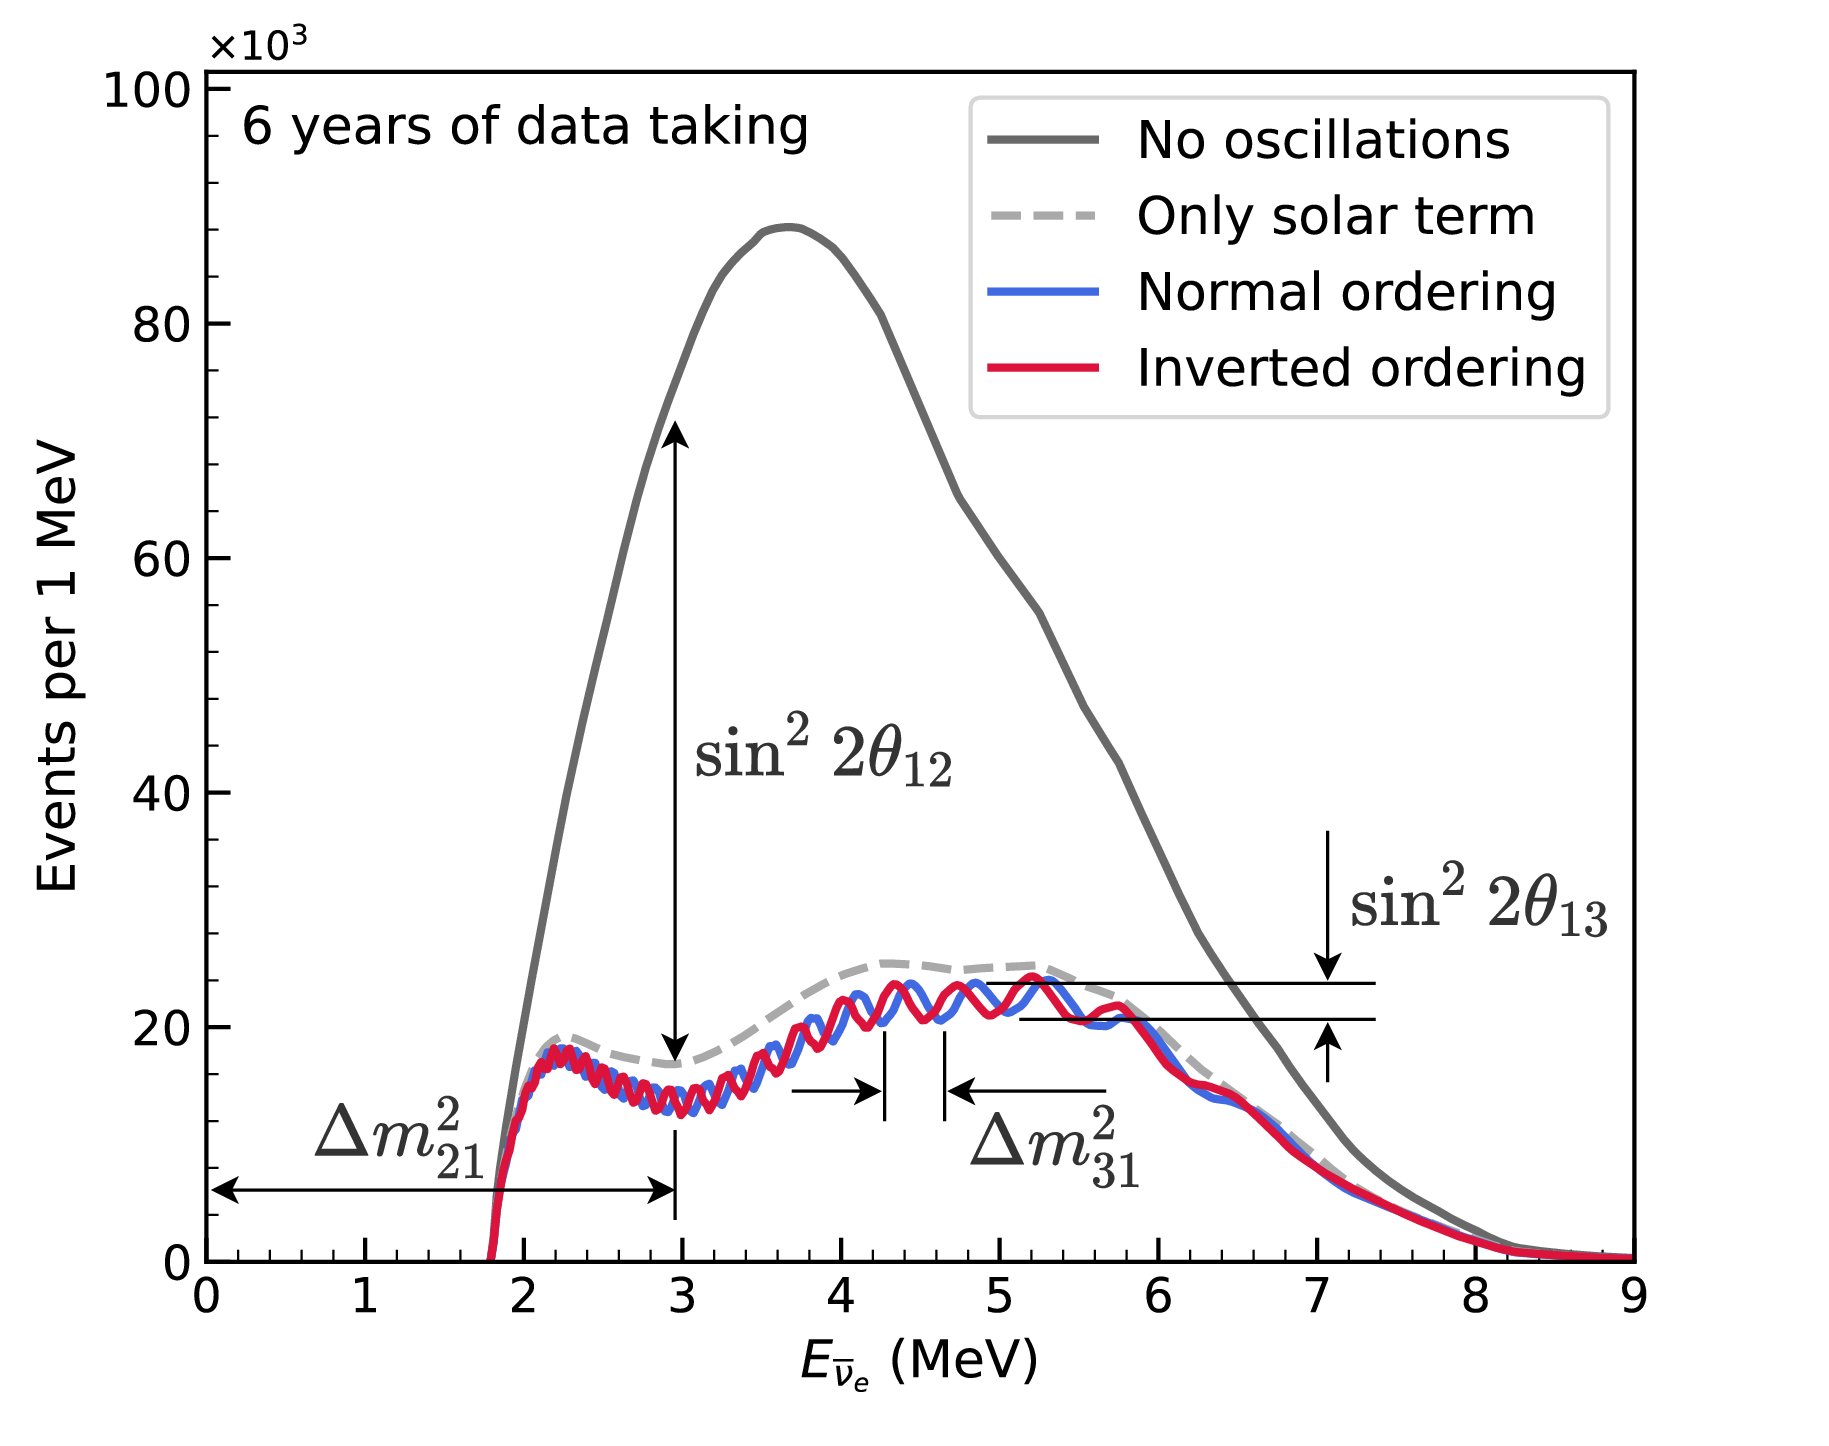
\includegraphics[height=8cm]{images/juno/Spectrum-OscillationsOnly_dm2_31.png}
  \caption{Expected number of neutrinos event per MeV in JUNO after 6 years of data taking. The black curve shows the flux if there was no oscillation. The light gray curve shows the oscillation if only the solar terms are taken in account ($\theta_{12}$, $\Delta m_{21}^2$. The blue and red curve shows the spectrum in the case of, respectively, NO and IO. The dependency of the oscillation to the different parameters are schematized by the double sided arrows. We can see the NMO sensitivity by looking at the fine phase shift between the red and the blue curve.}
  \label{fig:juno-spectrum-oscillation}
\end{figure}

\subsubsection{Identification of the mass hierarchy}

\todo{Continue here using 2.3 of Neutrino Physics with JUNO}

\subsubsection{Precise measurement of the oscillations parameters}

\subsection{Other physics}

\subsubsection{Geoneutrinos}

\subsubsection{Atmospheric neutrinos}

\subsubsection{Beyond standard model neutrinos interactions}

\subsubsection{Supernovae burst neutrinos}

\subsubsection{Diffuse supernovae neutrinos background}

\subsubsection{Background in the neutrinos reactor spectrum}

\section{The JUNO detector}

\subsection{Central Detector (CD)}

\subsubsection{Acrylic containment sphere}

\subsubsection{Liquid scintillator}

\subsubsection{Large photo-multipliers (LPMTs)}

\subsubsection{Small photo-multipliers (SPMTs)}

\subsubsection{Data Acquisition System (DAQ)}

\subsubsection{Simulation}

\subsubsection{Software}

\todo{Expliquer comment le software fonctionne}


\subsection{Veto detector}

\subsubsection{Cherenkov in water pool}

\subsubsection{Top tracker}

\section{Calibration strategy}

\subsection{Energy scale calibration}

\subsection{Calibration system}

\subsection{Calibration program}

\section{Event selection and background rejection}

\todo{Explication de comment reconnaitre un IDB (OEC)}

\subsection{Fiducial volume}

\subsection{Muon tagging}

\section{State of the art of the IBD reconstruction}

\subsection{Interaction vertex reconstruction}

\subsection{Energy reconstruction}

\subsection{Particle identification}

\subsection{Machine learning for reconstruction}

\subsubsection{Vertex reconstruction}

\subsubsection{Energy reconstruction}

\section{JUNO sensitivity to NMO and precise measurements}

\subsection{Fitting procedure}
